\documentclass{standalone}
\usepackage{pgfplots}
\begin{document}

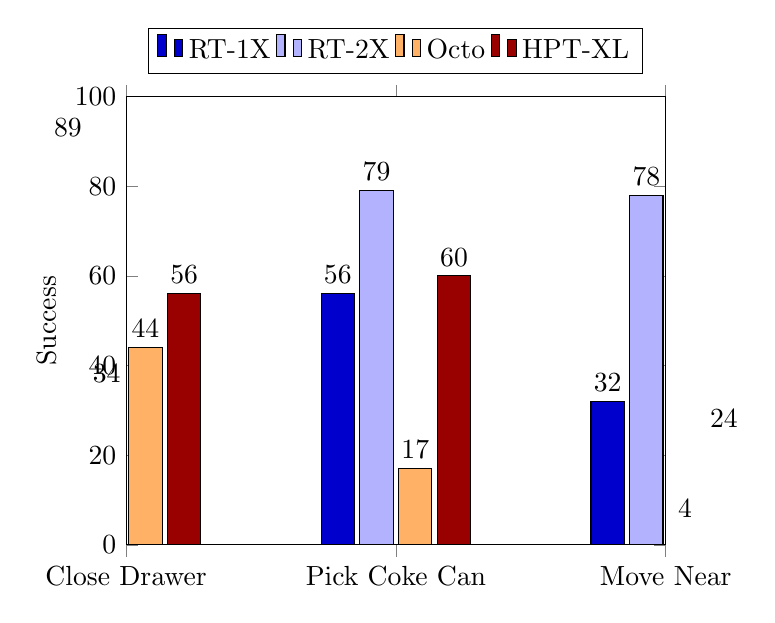
\begin{tikzpicture}
\begin{axis}[
    ybar,
    bar width=12pt,
    enlargelimits=-0.15,
    legend style={at={(0.5,1.05)}, anchor=south,legend columns=-1},
    legend cell align=left,
    symbolic x coords={Close Drawer,Pick Coke Can,Move Near},
    xtick=data,
    ylabel={Success},
    ymin=0, ymax=100,
    nodes near coords,
    nodes near coords align={vertical},
]
\addplot[fill=blue!80!black] coordinates {(Close Drawer,89) (Pick Coke Can,56) (Move Near,32)};
\addplot[fill=blue!30] coordinates {(Close Drawer,34) (Pick Coke Can,79) (Move Near,78)};
\addplot[fill=orange!60] coordinates {(Close Drawer,44) (Pick Coke Can,17) (Move Near,4)};
\addplot[fill=red!60!black] coordinates {(Close Drawer,56) (Pick Coke Can,60) (Move Near,24)};
\legend{RT-1X, RT-2X, Octo, HPT-XL}
\end{axis}
\end{tikzpicture}

\end{document}